\documentclass[../TDT5.tex]{subfiles}%

\begin{document}
\section{Moteur Diesel à double combustion}
\enonce{%
	Dans les moteurs Diesel à double combustion, le cycle décrit par le mélange
	air-carburant est modélisable par celui d'un système fermé représenté en
	coordonnées de \textsc{Watt} ci-après.
	\smallbreak
	\noindent
	\begin{minipage}[c]{.25\linewidth}
		\begin{center}
			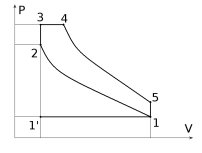
\includegraphics[width=\linewidth]{E6_cycle_diesel}
		\end{center}
	\end{minipage}
	\hfill
	\noindent
	\begin{minipage}[c]{.70\linewidth}
		Après la phase d'admission $1' \to 1$ qui amène le mélange au point 1 du
		cycle, celui-ci subit une compression adiabatique supposée réversible
		jusqu'au point 2. Après injection du carburant en 2, la combustion
		s'effectue d'abord de façon isochore de 2 à 3 puis se poursuit de façon
		isobare de 3 à 4. La phase de combustion est suivie d'une détente
		adiabatique à nouveau prise réversible de 4 à 5, puis d'une phase
		d'échappement isochore $5 \to 1$ puis isobare $1 \to 1'$.
	\end{minipage}
	Au point 1 du cycle, la pression $p_m = \SI{1.0}{bar}$ et la température $T_m
		= \SI{293}{K}$ sont minimales. La pression maximale, aux points 3 et 4, est
	$p_M = \SI{60}{bar}$ et la température maximale, au point 4, vaut $T_M =
		\SI{2073}{K}$. Le rapport volumétrique de compression vaut $\beta = V_M/V_m =
		\num{17}$.
	\smallbreak
	On suppose que le mélange air-carburant se comporte exactement comme l'air,
	c'est-à-dire comme un gaz parfait diatomique de masse molaire $M =
		\SI{29}{g.mol^{-1}}$, et de capacités thermiques respectives $C_P$ et $C_V$.
}%
\QR{%
	Exprimer les températures $T_2$, $T_3$ et $T_5$ en fonction de $p_m$, $p_M$,
	$T_m$, $T_M$ et $\beta$. Calculer les valeurs numériques.
}{%
	La transformation $1\to 2$ est une adiabatique réversible (donc isentropique)
	d'un gaz parfait~; d'après la loi de \textsc{Laplace} en température et volume
	$TV^{\gamma-1} = \cte$, on a
	\[
		T_2 = T_1 \left( \frac{V_1}{V_2} \right)^{\gamma-1}
		\Lra
		\boxed{T_2 = \beta^{\gamma-1}T_m}
		\Ra
		\xul{T_2 = \SI{9.1e2}{K}}
	\]
	La transformation $2\to 3$ est isochore, d'où par l'équation d'état
	\begin{gather*}
		\frac{P_3}{T_3} = \frac{P_2}{T_2}
		\qav
		\left\{
		\begin{array}{rcl}
			T_2 & = & \beta^{\gamma-1}T_m
			\\
			P_3 & = & P_m
			\\
			P_2 & = & \left( \frac{V_1}{V_2} \right)^{\gamma}P_1 = \beta^{\gamma}P_m
		\end{array}
		\right.\\
		\AN
		\boxed{
			T_3 = \frac{P_M}{\beta P_m}T_m
		}
		\Ra
		\xul{T_3 = \SI{1.0e3}{K}}
	\end{gather*}
	Enfin, la loi de \textsc{Laplace} appliquée sur $4\to 5$ qui est isentropique
	donne
	\begin{gather*}
		T_5 = \left( \frac{V_4}{V_5} \right)^{\gamma}T_4
		\qor
		\frac{V_4}{T_4} \stc{=}{\text{isoP}} \frac{V_3}{T_3}
		\\\Ra
		T_5 =
		\left( \frac{V_3}{V_5}\frac{T_4}{T_3} \right)^{\gamma}T_4 =
		\left( \frac{1}{\beta}\frac{T_M}{T_m}\frac{\beta P_m}{P_M}
		\right)^{\gamma}T_M
		\\\Lra
		\boxed{T_5 = \left( \frac{T_MP_m}{T_mP_M} \right)^{\gamma}T_M}
		\Ra
		\xul{T_5 = \SI{8.8e2}{K}}
	\end{gather*}
}%
\QR{%
	Calculer le transfert thermique massique $q_C$ reçu par l'air au cours de la
	phase de combustion $2 \to 4$.
}{%
	Notons $n$ la quantité de matière de gaz du mélange. Le transfert thermique
	$Q_C$ est fourni au cours des étapes $2\to 3$ est $3\to 4$. En utilisant d'une
	part le bilan d'énergie (premier principe) sur $2\to 3$ isochore et le fait
	que le système soit un gaz parfait, on trouve
	\[
		\Delta{U}_{23} \stc{=}{\text{1\ier{} ppe.}} \underbracket[1pt]{W_{23}}_{=0} + Q_{23}
		\qet
		\Delta{U}_{23} \stc{=}{\text{G.P.}} C_V \Delta{T}_{23} = \frac{nR}{\gamma-1}(T_3-T_2)
	\]
	De même, pour $3\to 4$ qui est isobare donc pour laquelle on applique le
	premier principe enthalpique,
	\[
		\Delta{H}_{34} \stc{=}{\text{1\ier{} ppe.}} \underbracket[1pt]{W_{u,34}}_{=0} + Q_{34}
		\qet
		\Delta{H}_{34} \stc{=}{\text{G.P.}} C_P \Delta{T}_{34} = \frac{\gamma nR}{\gamma-1}(T_4-T_3)
	\]
	Puis en introduisant $m$ \textit{via} $n = m/M$~:
	\begin{gather*}
		Q_C = Q_{23} + Q_{34} = \Delta{U}_{23} + \Delta{H}_{34}
		\qso
		Q_C = \frac{mR}{M (\gamma-1)} [T_3-T_2 + \gamma (T_4-T_3)]
		\\\Lra
		\boxed{q_C = \frac{R}{M (\gamma-1)} [T_3-T_2 + \gamma (T_4-T_3)]}
		\Ra
		\xul{q_C = \SI{1.1e3}{kJ.kg^{-1}}}
	\end{gather*}
}%
\QR{%
	Calculer le transfert thermique massique $q_F$ échangé avec le milieu
	extérieur entre les points $5$ et $1$.
}{%
	Comme $5\to 1$ est isochore d'un gaz parfait, on a
	\begin{gather*}
		\Delta{U}_{5\to 1} \stc{=}{\text{1\ier{} ppe.}} Q_{51}
		\qet
		\Delta{U}_{5\to 1} \stc{=}{\text{G.P.}} \frac{nR}{\gamma-1} (T_1-T_5)
		\\\Ra
		\boxed{q_F = \frac{R}{M (\gamma-1)}(T_1-T_5)}
		\Ra
		\xul{q_F = \SI{-4.2e2}{kJ.kg^{-1}}}
	\end{gather*}
}%
\QR{%
	En déduire le travail massique $w$ échangé au cours d'un cycle.
}{%
	D'après le premier principe appliqué à l'ensemble du cycle,
	\[
		W = -Q_F - Q_C
		\Lra
		\boxed{w = -q_F - q_C}
		\Ra
		\xul{w = \SI{-7.1e2}{kJ.kg^{-1}}}
	\]
}%
\QR{%
	Définir et calculer le rendement de ce moteur. Commenter la valeur trouvée.
}}
	\]
	C'est une valeur élevée, mais qui a été obtenue avec une modélisation très
	idéalisée des transformations. En pratique, l'ordre de grandeur du rendement
	d'un moteur diesel est plutôt de \numrange{40}{45}\%.
}%

\end{document}
